\documentclass[tikz,border=6pt]{standalone}

\usepackage{xcolor}
\usetikzlibrary{arrows.meta}

\begin{document}

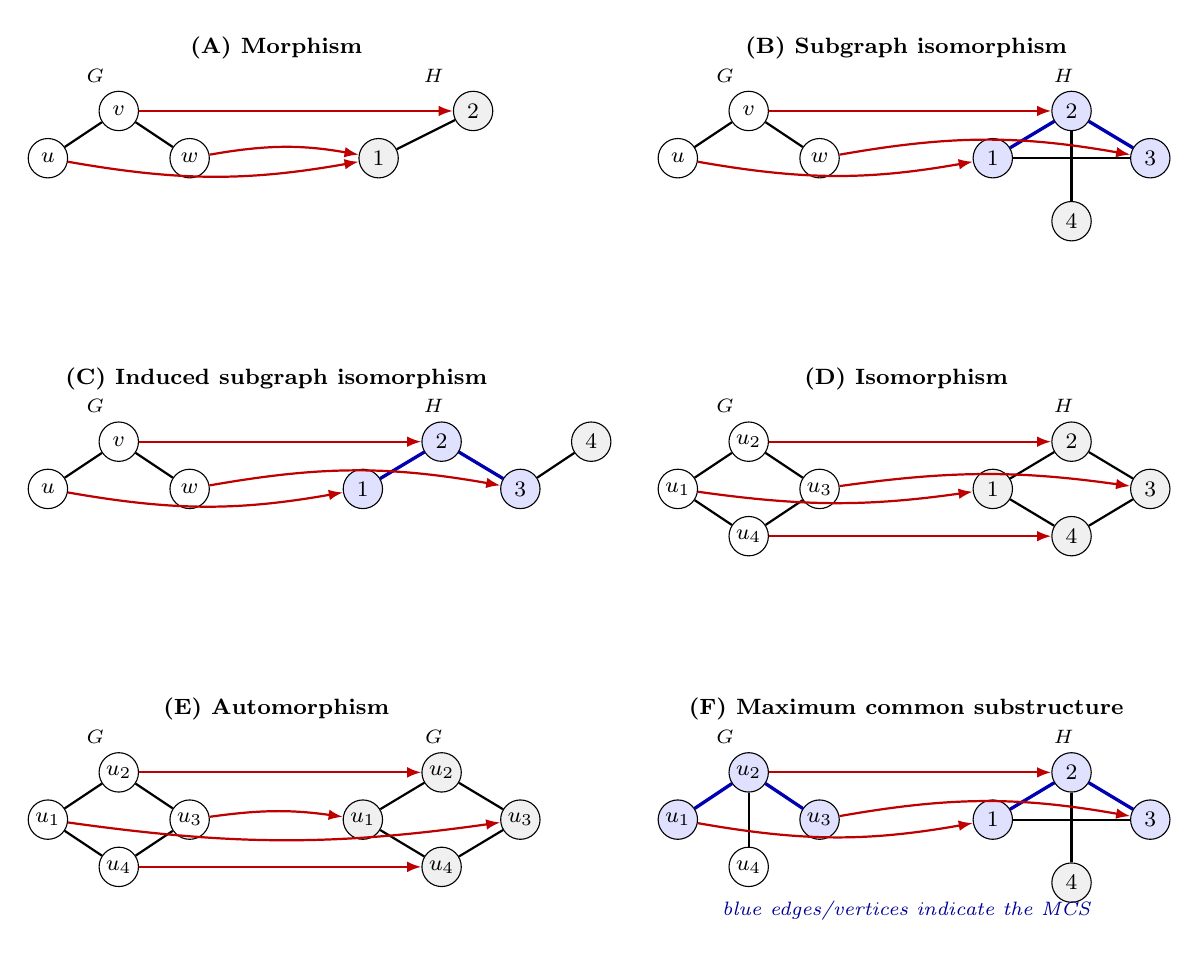
\begin{tikzpicture}[
  x=1cm,y=1cm,
  font=\footnotesize,
  vG/.style={circle,draw,fill=white,minimum size=5mm,inner sep=1pt},
  vH/.style={circle,draw,fill=gray!12,minimum size=5mm,inner sep=1pt},
  vI/.style={circle,draw,fill=blue!12,minimum size=5mm,inner sep=1pt},
  e/.style={thick},
  img/.style={very thick,blue!70!black},
  map/.style={-{Latex[length=1.8mm]},red!75!black,thick},
  title/.style={font=\bfseries\footnotesize},
  graphlabel/.style={font=\scriptsize},
  mcsnote/.style={font=\scriptsize\itshape, text=blue!60!black}
]

% Layout:
% Row 1: A, B
% Row 2: C, D
% Row 3: E, F

%%%%%%%%%%%%%%%%%%%%%%%%%%%%%%%%%%%%%%%%%%%%%%%%%%%%
% (A) Morphism
%%%%%%%%%%%%%%%%%%%%%%%%%%%%%%%%%%%%%%%%%%%%%%%%%%%%
\begin{scope}[shift={(0,0)}]
\node[title] at (2.9,2.1) {(A) Morphism};

\node[graphlabel] at (0.6,1.75) {$G$};
\node[vG] (AG1) at (0,0.7) {$u$};
\node[vG] (AG2) at (0.9,1.3) {$v$};
\node[vG] (AG3) at (1.8,0.7) {$w$};
\draw[e] (AG1)--(AG2)--(AG3);

\node[graphlabel] at (4.9,1.75) {$H$};
\node[vH] (AH1) at (4.2,0.7) {$1$};
\node[vH] (AH2) at (5.4,1.3) {$2$};
\draw[e] (AH1)--(AH2);

\draw[map] (AG1) to[bend right=10] (AH1);
\draw[map] (AG2) -- (AH2);
\draw[map] (AG3) to[bend left=10] (AH1);
\end{scope}

%%%%%%%%%%%%%%%%%%%%%%%%%%%%%%%%%%%%%%%%%%%%%%%%%%%%
% (B) Subgraph isomorphism
%%%%%%%%%%%%%%%%%%%%%%%%%%%%%%%%%%%%%%%%%%%%%%%%%%%%
\begin{scope}[shift={(8,0)}]
\node[title] at (2.9,2.1) {(B) Subgraph isomorphism};

\node[graphlabel] at (0.6,1.75) {$G$};
\node[vG] (BG1) at (0,0.7) {$u$};
\node[vG] (BG2) at (0.9,1.3) {$v$};
\node[vG] (BG3) at (1.8,0.7) {$w$};
\draw[e] (BG1)--(BG2)--(BG3);

\node[graphlabel] at (4.9,1.75) {$H$};
\node[vI] (BH1) at (4.0,0.7) {$1$};
\node[vI] (BH2) at (5.0,1.3) {$2$};
\node[vI] (BH3) at (6.0,0.7) {$3$};
\node[vH] (BH4) at (5.0,-0.1) {$4$};

\draw[e] (BH1)--(BH2)--(BH3);
\draw[e] (BH1)--(BH3);    % extra edge: not induced
\draw[e] (BH2)--(BH4);
\draw[img] (BH1)--(BH2)--(BH3);

\draw[map] (BG1) to[bend right=10] (BH1);
\draw[map] (BG2) -- (BH2);
\draw[map] (BG3) to[bend left=10] (BH3);
\end{scope}

%%%%%%%%%%%%%%%%%%%%%%%%%%%%%%%%%%%%%%%%%%%%%%%%%%%%
% (C) Induced subgraph isomorphism
%%%%%%%%%%%%%%%%%%%%%%%%%%%%%%%%%%%%%%%%%%%%%%%%%%%%
\begin{scope}[shift={(0,-4.2)}]
\node[title] at (2.9,2.1) {(C) Induced subgraph isomorphism};

\node[graphlabel] at (0.6,1.75) {$G$};
\node[vG] (CG1) at (0,0.7) {$u$};
\node[vG] (CG2) at (0.9,1.3) {$v$};
\node[vG] (CG3) at (1.8,0.7) {$w$};
\draw[e] (CG1)--(CG2)--(CG3);

\node[graphlabel] at (4.9,1.75) {$H$};
\node[vI] (CH1) at (4.0,0.7) {$1$};
\node[vI] (CH2) at (5.0,1.3) {$2$};
\node[vI] (CH3) at (6.0,0.7) {$3$};
\node[vH] (CH4) at (6.9,1.3) {$4$};

\draw[e] (CH1)--(CH2)--(CH3)--(CH4);
\draw[img] (CH1)--(CH2)--(CH3);

\draw[map] (CG1) to[bend right=10] (CH1);
\draw[map] (CG2) -- (CH2);
\draw[map] (CG3) to[bend left=10] (CH3);
\end{scope}

%%%%%%%%%%%%%%%%%%%%%%%%%%%%%%%%%%%%%%%%%%%%%%%%%%%%
% (D) Isomorphism
%%%%%%%%%%%%%%%%%%%%%%%%%%%%%%%%%%%%%%%%%%%%%%%%%%%%
\begin{scope}[shift={(8,-4.2)}]
\node[title] at (2.9,2.1) {(D) Isomorphism};

\node[graphlabel] at (0.6,1.75) {$G$};
\node[vG] (DG1) at (0,0.7) {$u_1$};
\node[vG] (DG2) at (0.9,1.3) {$u_2$};
\node[vG] (DG3) at (1.8,0.7) {$u_3$};
\node[vG] (DG4) at (0.9,0.1) {$u_4$};
\draw[e] (DG1)--(DG2)--(DG3)--(DG4)--(DG1);

\node[graphlabel] at (4.9,1.75) {$H$};
\node[vH] (DH1) at (4.0,0.7) {$1$};
\node[vH] (DH2) at (5.0,1.3) {$2$};
\node[vH] (DH3) at (6.0,0.7) {$3$};
\node[vH] (DH4) at (5.0,0.1) {$4$};
\draw[e] (DH1)--(DH2)--(DH3)--(DH4)--(DH1);

\draw[map] (DG1) to[bend right=8] (DH1);
\draw[map] (DG2) -- (DH2);
\draw[map] (DG3) to[bend left=8] (DH3);
\draw[map] (DG4) -- (DH4);
\end{scope}

%%%%%%%%%%%%%%%%%%%%%%%%%%%%%%%%%%%%%%%%%%%%%%%%%%%%
% (E) Automorphism
%%%%%%%%%%%%%%%%%%%%%%%%%%%%%%%%%%%%%%%%%%%%%%%%%%%%
\begin{scope}[shift={(0,-8.4)}]
\node[title] at (2.9,2.1) {(E) Automorphism};

\node[graphlabel] at (0.6,1.75) {$G$};
\node[vG] (EG1) at (0,0.7) {$u_1$};
\node[vG] (EG2) at (0.9,1.3) {$u_2$};
\node[vG] (EG3) at (1.8,0.7) {$u_3$};
\node[vG] (EG4) at (0.9,0.1) {$u_4$};
\draw[e] (EG1)--(EG2)--(EG3)--(EG4)--(EG1);

\node[graphlabel] at (4.9,1.75) {$G$};
\node[vH] (EH1) at (4.0,0.7) {$u_1$};
\node[vH] (EH2) at (5.0,1.3) {$u_2$};
\node[vH] (EH3) at (6.0,0.7) {$u_3$};
\node[vH] (EH4) at (5.0,0.1) {$u_4$};
\draw[e] (EH1)--(EH2)--(EH3)--(EH4)--(EH1);

\draw[map] (EG1) to[bend right=8] (EH3);
\draw[map] (EG2) -- (EH2);
\draw[map] (EG3) to[bend left=8] (EH1);
\draw[map] (EG4) -- (EH4);
\end{scope}

%%%%%%%%%%%%%%%%%%%%%%%%%%%%%%%%%%%%%%%%%%%%%%%%%%%%
% (F) Maximum common substructure
%%%%%%%%%%%%%%%%%%%%%%%%%%%%%%%%%%%%%%%%%%%%%%%%%%%%
\begin{scope}[shift={(8,-8.4)}]
\node[title] at (2.9,2.1) {(F) Maximum common substructure};

\node[graphlabel] at (0.6,1.75) {$G$};
\node[vI] (FG1) at (0,0.7) {$u_1$};
\node[vI] (FG2) at (0.9,1.3) {$u_2$};
\node[vI] (FG3) at (1.8,0.7) {$u_3$};
\node[vG] (FG4) at (0.9,0.1) {$u_4$};
\draw[e] (FG1)--(FG2)--(FG3);
\draw[e] (FG2)--(FG4);
\draw[img] (FG1)--(FG2)--(FG3);

\node[graphlabel] at (4.9,1.75) {$H$};
\node[vI] (FH1) at (4.0,0.7) {$1$};
\node[vI] (FH2) at (5.0,1.3) {$2$};
\node[vI] (FH3) at (6.0,0.7) {$3$};
\node[vH] (FH4) at (5.0,-0.1) {$4$};
\draw[e] (FH1)--(FH2)--(FH3);
\draw[e] (FH1)--(FH3);
\draw[e] (FH2)--(FH4);
\draw[img] (FH1)--(FH2)--(FH3);

\draw[map] (FG1) to[bend right=10] (FH1);
\draw[map] (FG2) -- (FH2);
\draw[map] (FG3) to[bend left=10] (FH3);

\node[mcsnote] at (2.9,-0.45) {blue edges/vertices indicate the MCS};
\end{scope}

\end{tikzpicture}

\end{document}